% Main file

\documentclass[a4paper,11pt]{article}   % list options between brackets
\usepackage[style=numeric,backend=bibtex]{biblatex}
\addbibresource{references.bib}
% Include configuration (loading packages, defining the style of the document...)
% Important packages

\usepackage[margin=1.7in]{geometry}
\usepackage[francais,english]{babel}
\usepackage[utf8]{inputenc}
%\usepackage[T1]{fontenc}
\usepackage{acronym}
\usepackage{graphicx}
\usepackage{hyperref}
\usepackage{xcolor}
\usepackage{amsmath}
\usepackage{eurosym}
\usepackage{lipsum}
\usepackage{multicol}
\usepackage{multirow}
\usepackage{booktabs}
\usepackage[inline]{enumitem}
\usepackage{fancyhdr}
\usepackage{algorithm}
\usepackage[noend]{algpseudocode}
\floatname{algorithm}{Pseudocode}
\usepackage{subcaption}


	  



% Include user's macros
% Math macros
\newcommand*{\SET}[1]  {\ensuremath{\mathrm{\mathbf{#1}}}}
\newcommand*{\VEC}[1]  {\ensuremath{\boldsymbol{#1}}}
\newcommand*{\MAT}[1]  {\ensuremath{\boldsymbol{#1}}}
\newcommand*{\OP}[1]  {\ensuremath{\boldsymbol{\mathcal{#1}}}}
\newcommand*{\ESP}[1]  {\ensuremath{ \mathbb{E} \left \{#1 \right \}}}
\newcommand*{\ESPENS}[2]  {\ensuremath{ \mathbb{E}_{#1} \left \{#2 \right \}}}
\newcommand*{\NORM}[1]  {\ensuremath{\left\|#1\right\|}}
\newcommand*{\DPR}[2]  {\ensuremath{\left \langle #1,#2 \right \rangle}}
\newcommand*{\FOURIER}[1]  {\ensuremath{\widehat{#1}}}
\newcommand{\eqdef}{\stackrel{\mathrm{def}}{=}}
\newcommand{\argmax}{\operatornamewithlimits{argmax}}
\newcommand{\argmin}{\operatornamewithlimits{argmin}}
\newcommand{\diag}{\operatorname{diag}}
\newcommand{\ud}{\, \mathrm{d}}
\newcommand{\vect}{\mathrm{Vect}}
\newcommand{\sinc}{\mathrm{sinc}}
\newcommand{\esp}{\ensuremath{\mathrm{E}}} % Problème pour les short captions
\newcommand{\hilbert}{\ensuremath{\mathcal{H}}}
\newcommand{\supps}{\ensuremath{\tilde{\mathrm{supp}}}}
\newcommand{\supp}{\ensuremath{\mathrm{supp}}}
\newcommand{\sgn}{\mathrm{sgn}}
\newcommand{\intTT}{\int_{-T}^{T}}
\newcommand{\intT}{\int_{-\frac{T}{2}}^{\frac{T}{2}}}
\newcommand{\intinf}{\int_{-\infty}^{+\infty}}
\newcommand{\iintinf}{\iint_{-\infty}^{+\infty}}
\newcommand{\iintrr}{\iint\limits_{\SET{R}^2}}
\newcommand{\intr}{\int\limits_{\R}}
\newcommand{\Sh}{\ensuremath{\boldsymbol{U}}}
\newcommand{\C}{\ensuremath{\mathbf{C}}}
\newcommand{\R}{\ensuremath{\mathbf{R}}}
\newcommand{\Z}{\ensuremath{\mathbf{Z}}}
\newcommand{\N}{\ensuremath{\mathbf{N}}}
\newcommand{\K}{\ensuremath{\mathbf{K}}}
\newcommand{\reel}{\mathcal{R}}
\newcommand{\imag}{\mathcal{I}}
\newcommand{\cmnr}{c_{m,n}^\reel}
\newcommand{\cmni}{c_{m,n}^\imag}
\newcommand{\cnr}{c_{n}^\reel}
\newcommand{\cni}{c_{n}^\imag}
\newcommand{\tproto}{g}
\newcommand{\rproto}{\check{g}}
\newcommand{\Tproto}{G}
\newcommand{\Rproto}{\check{G}}
\newcommand{\Tpoly}{F}
\newcommand{\Rpoly}{\check{F}}
\newcommand{\estim}{\tilde{c}}
\newcommand{\egal}{\bar{c}}
\newcommand{\bb}{b}
\newcommand{\bbf}{z}
\newcommand{\bbr}{\zeta}
\newcommand{\LR}{\mathcal{L}_2(\R)}
\newcommand{\LRR}{\mathcal{L}_2(\R^2)}
\newcommand{\LZ}{\ell_2(\Z)}
\newcommand{\LZZ}{\ell_2(\Z^2)}
\newcommand{\peigne}{\ensuremath{\Psi}}
\newcommand{\avec}{\qquad \text{avec} \qquad}


%%%%%%%%%%%% Head and foot Texts

\pagestyle{fancy}
\fancyhf{}
\lhead{ND2I Project - Capgemini Engineering}
\fancyfoot[L]{Author: Sana IKLI}
\fancyfoot[R]{\thepage}



\begin{document}
	% Include the title pages
	%%%%%%%%%%%%%%%%%%%%     Title page      %%%%%%%%%%%%%%%%%%%%%%
\begin{titlepage}
	\begin{center}
		\vspace*{1cm}
		
		
\includegraphics[width=.95\textwidth]{images/cap-logo}
		
		
		\vspace*{3.4cm}
        \begin{center}
		\rule{12cm}{1.4pt}
		\end{center}
		
		\textbf{\MakeUppercase{How to manage a fleet of flying taxis in a dynamic environment}}
		
		\vspace{0.3cm}
		\textsc{FINAL DELIVERABLE}\\
		
		\vspace{0.6cm}
		ND2I Project\\
		Deliverable Document
		\begin{center}
			\rule{8cm}{1.2pt}
		\end{center}


		\vspace{1cm}

		{\large\textsc{sana ikli}}\\
		\today
		
		\vspace{4cm}
		\hfill\og\textit{Knowledge is wasted when it isn't shared.}\fg
		
	\end{center}
	\end{titlepage}	
%%%%%%%%%%%%%%%%%%%%%%%%%%%%%%%%%%%%%%%%%%%%%%%%%%%%%%%%%%%
	

	
	%%%%%%%%%%%%%%%%%%%%%%%%%%
	%%% Sections are included here 
	%%%%%%%%%%%%%%%%%%%%%%%%%%
	
% Section 0

\section*{Abstract}

abstract here...

abstract here...

abstract here...

abstract here...

abstract here...

abstract here...

abstract here...


% First section

\section{Introduction}


Flying taxis are expected to serve as an alternative to ground transportation to alleviate traffic congestion in metropolitan cities. Several transportation pioneers and airline manufacturers are preparing to launch their Urban Air Mobility (\acs{UAM}) services in the near future. Indeed, Airbus Helicopters is currently working on new electric flying taxis as a part of the \textit{CityAirbus Nextgen} project~\cite{airbus2025}. Their flying taxis are expected to operate in 2025. Apart from Airbus, Uber is also working on an air taxi service called \textit{Uber Elevate}, which is estimated to lunch in 2023~\cite{rajendran2019}.

Due to the dynamic nature of the problem, the companies proposing air taxi service will deal with several real-time decisions. Such decisions include
\begin{enumerate*}[label=(\roman*)]
	\item evaluating different candidate trips and scheduling the flying taxis so as to optimize a given objective (\textit{e.g.}, reduce the operational costs, serve the maximum number of demands, etc.),
	\item dynamic estimation of the market demands, and
	
	\item battery charging management as well as other maintenance related-issues~\cite{rajendran2020}.
\end{enumerate*}

In this work, we are interested in the real-time management of a fleet of flying taxis. The management includes the dynamic scheduling of the air taxis and the battery charging handling. This work is one of the few that considers the (more realistic) real-time problem, where decisions have to be made dynamically to accommodate the new changes in the air taxi environment. 

A common strategy used in the literature to tackle the dynamic scheduling is the \textit{Rolling Horizon} (\acs{RH}) approach. The latter usually subdivides the scheduling horizon into smaller sub-horizons, and then it solves the static problem on each sub-horizon. These strategies are used in the literature to tackle (the dynamic version of) two well-know optimization problem that are \emph{similar} to our problem, namely: the Job-Shop Scheduling Problem (\acs{JSSP}) and the Vehicle Routing Problem (\acs{VRP}). 

The analogy between a \acs{JSSP} and the scheduling of air taxis can be described as follows. The machines represent the flying taxis, and the jobs represent the demands. The trip duration of a given demand can be interpreted as the processing time of a job in the \acs{JSSP} framework. A fundamental aspect of the flying taxis framework is the battery charging; the latter can be translated to the \acs{JSSP} model as the machine breakdown, \textit{i.e.,} a specified period of time during which a machine is is out of order.

In addition, the scheduling of air taxis is clearly similar to the \acs{VRP}. In the two frameworks, we have vehicles to dispatch and clients to serve. The battery charging of an air taxi is translated to the VRP framework as the vehicle refueling.

As a consequence of these analogies, we can derive two conclusions. On the one hand, the problem of scheduling flying taxis, the \acs{JSSP}, and the \acs{VRP} have the same complexity: they are NP-hard problems (\acs{JSSP} and the \acs{VRP} are already proven to be NP-hard~\cite{mohan2019,song2016}). On the other hand, we can use the literature of the dynamic \acs{JSSP} and the \acs{VRP} to gain insights on how the real-time problems are handled. The latter is the objective of the next section.



	
	% Second section

\section{Literature review: Dynamic scheduling techniques}

Rolling horizon approaches are common strategies in the literature to solve the dynamic scheduling problems. They generally consist in subdividing the planing horizon into smaller sub-horizons. Then solve the (static) problem on each sub-horizon sequentially, as illustrated in Figure~\ref{fig:rh}.
These approaches represent valid solution methods to tackle the dynamic case, because their computation times are usually suitable for real-time applications.

\begin{figure}[h!]
	\centering
	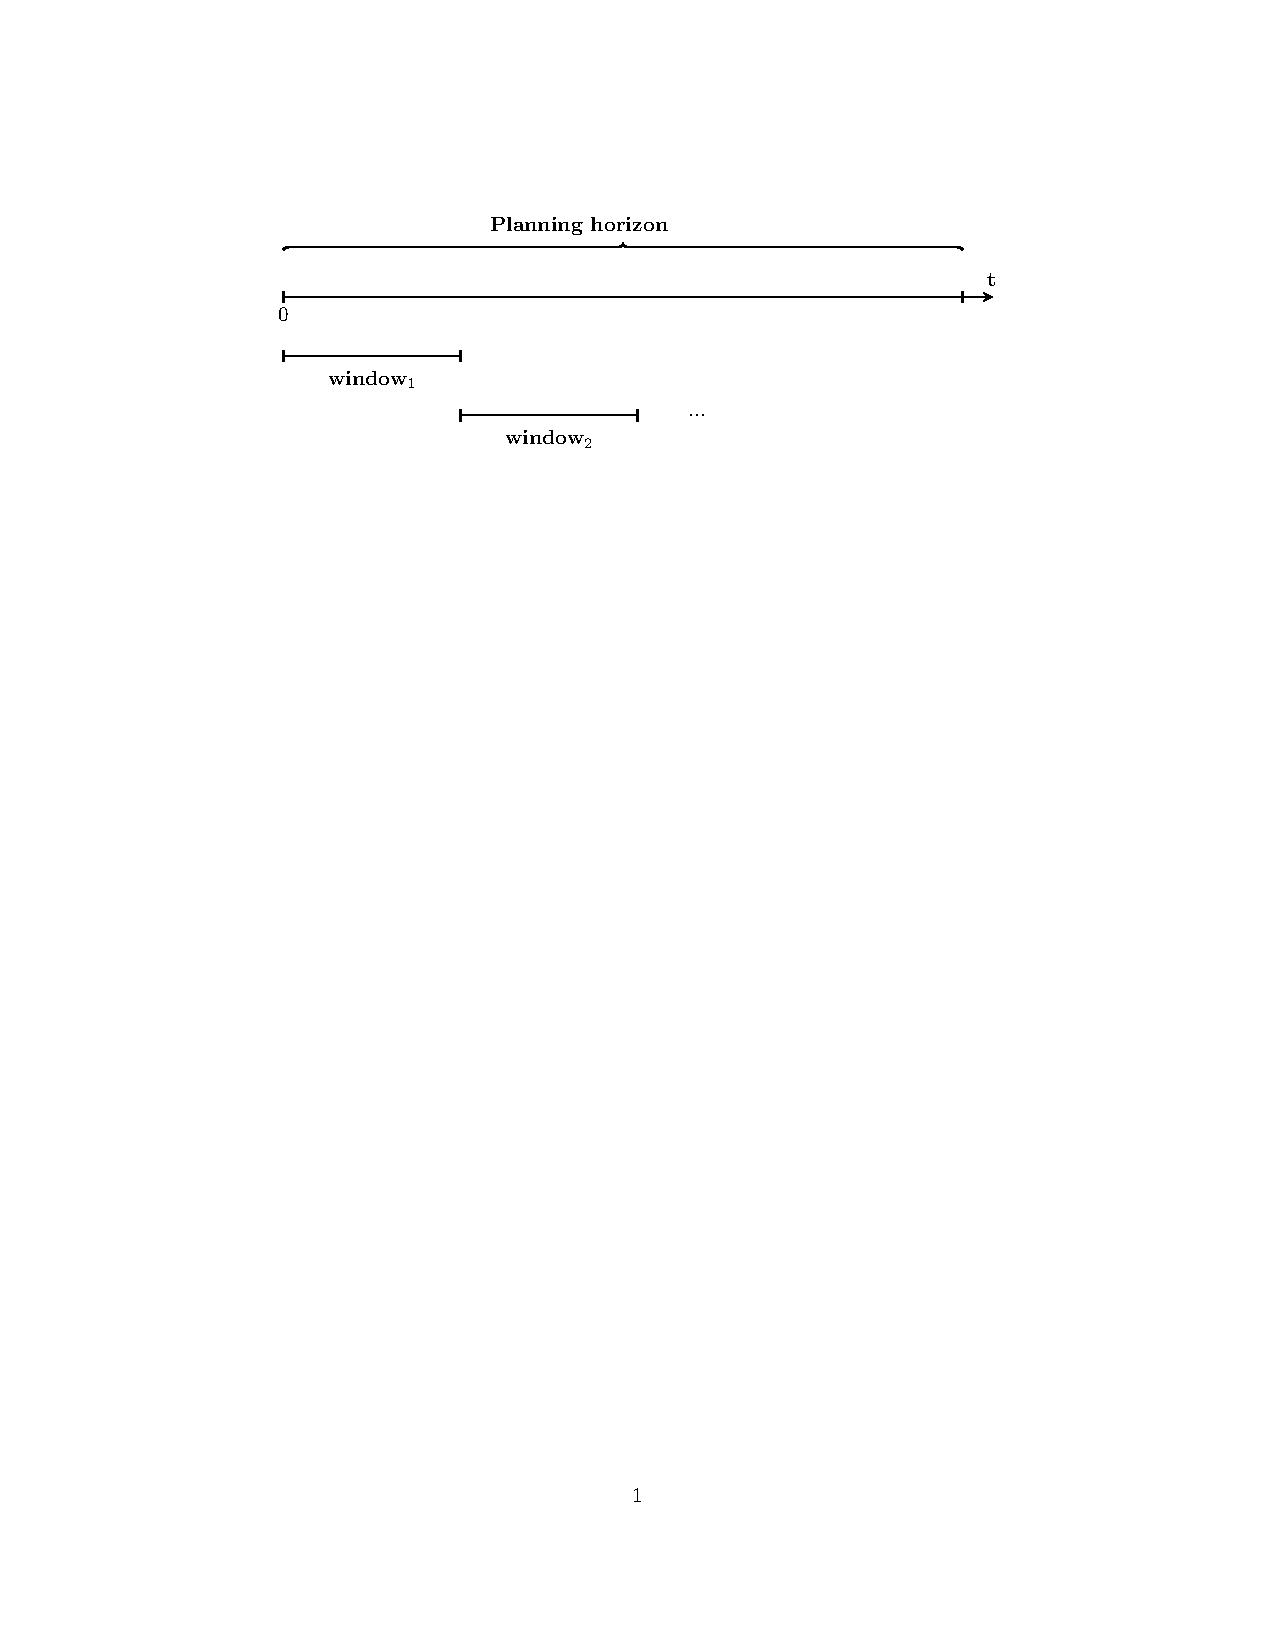
\includegraphics[trim=120 575 120 100,clip,width=0.85\textwidth]{images/rh.pdf}
	\caption{Illustration of the rolling-horizon approach.}
	\label{fig:rh}
\end{figure}
In the next subsection we review the most relevant \acs{RH} approaches for three optimization problems: the job-shop scheduling, the vehicle routing problem, and the unmanned ariel vehicle scheduling problem.


\subsection{Job-Shop Scheduling}
\label{subsec:machine}

In the \acs{RH} approaches for the Job-Shop Scheduling Problem (\acs{JSSP}), there are jobs that will start inside a sub-horizon and finish outside that horizon, regardless of its length. This kind of jobs is called \textit{cross-window} jobs. To deal with them, boundary conditions have to be defined for each sub-horizon. On the other hand, the computation complexity is expected to be reduced in the sub-horizons, since the problem size is smaller. The \acs{RH} scheduling approaches can be categorized into two types of strategies:

\begin{itemize}
	\item The \textit{event-driven} scheduling in which the rolling horizon is a job window, \textit{i.e.}, a number of jobs for scheduling and processing. This strategy first chooses a job window, which is defined by the (allowed) maximum number of jobs. Then, it divides the set of jobs in three sub-sets:
	\begin{enumerate*}[label=(\roman*)]
		\item the sub-set of available jobs,
		\item the sub-set of current jobs, and
		\item the sub-set of finished jobs.
	\end{enumerate*}
	
	A selection rule is then used to select jobs from the sub-set of available jobs. Finally, an optimization algorithm is required to solve the problem in the job windows, and the three above-mentioned sets are updated until all the jobs are processed. Notable examples from the literature that use this approach are~\cite{chen2017,fang1997}. The former work used this strategy to solve the online workflow scheduling on cloud environment, and the latter used it for the classical dynamic \acs{JSSP}.
	
	
	\item The \textit{periodic scheduling} strategies in which the rolling domain is a \textit{time window}, \textit{i.e.}, a time slot on the scheduling horizon. This strategy is used in~\cite{sun1994} to solve the dynamic JSSP. In this work, the authors subdivide the planning horizon, $T$, into two non-overlapping windows, $T_{1}$ and $T_{2}$. Then, they solve the (static) problem on $T_{2}$. Finally, they determine the set of cross-window jobs and schedules them with the jobs in the window $T_{1}$.  
	
	The periodic scheduling is also used in~\cite{tang2010}, but with a different \textit{rolling time-window}. In this context, the planning horizon, denoted $[0,K]$, is subdivided in $R$ time periods of equal lengths. Then, the problem is solved in the whole planing horizon at the beginning. As time progresses, the window is shortened by one time period, and the problem is again solved in the new window, as illustrated in Fig.~\ref{fig:tw-whole}.
	
	
	\begin{figure}[h!]
		\centering
		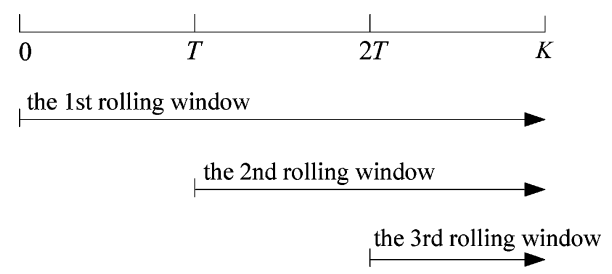
\includegraphics[width=.6\textwidth]{images/tw-whole}
		\caption{A rolling horizon with three time-windows (source:~\cite{tang2010}).}
		\label{fig:tw-whole}
	\end{figure}
	
\end{itemize}



\subsection{Vehicle Routing Problem}

In the dynamic \acs{VRP}, the customer orders are usually considered to be the dynamic events. In the work of Hanshar and Ombuki-Berman~\cite{hanshar2007}, the \acs{RH} periodic scheduling strategy is used, but with time-windows that differs from~\cite{sun1994} and~\cite{tang2010}. Indeed, in~\cite{hanshar2007} , the authors subdivide the planing horizons into several slices of equal lengths. Then, they sequentially solve the (static) VRP on each slice. Furthermore, the authors define a cutoff time, which postpones the late orders to the next day. The genetic algorithm is then used to solve the static problem on each time slice.

A number of heuristics are proposed in~\cite{larsen2002} to solve the dynamic VRP:

\begin{itemize}
	\item First-Come First-Served (FCFS) that serves the clients in the order which they are. A special case of this strategy is:
	
	\item Stochastic Queue Median (SQM) in which the vehicle travels directly from the median of the service region to the next demand location. After the service has been completed, the server returns to the median and waits for the next demand.
	
	\item Nearest Neighbor (NN) that completes the demands in one location, and then travels to the nearest neighboring demand.
\end{itemize}




\subsection{Unnamed Ariel Vehicle Scheduling}

The works in the literature addressing the real-time scheduling and routing of air taxis are rare compared to the machine scheduling or the VRP. Nonetheless, the two recent works~\cite{rajendran2021} and \cite{song2016} consider this dynamic scheduling for two types of air vehicles: the flying taxis for the former work, and the Unmanned Aerial Vehicle (\acs{UAV}) for the latter.

In\cite{song2016}, the authors develop a real-time tool to manage a fleet of \acs{UAV}s to serve customers. The management includes visiting the service station for battery recharging. The problem is formulated as a mixed-integer program, inspired from the \acs{VRP} literature, and solved using \textit{CPLEX}~\cite{cplex2009v12}. The dynamic scheduling is tackled using the \textit{event-driven} and the \textit{periodic scheduling} strategies explained in section~\ref{subsec:machine}.


In the very recent work of~\cite{rajendran2021}, the author considers the real-time dispatching of air taxis in a centralized taxi network. Two objectives are taken into account in the optimization model: minimizing  the \textbf{number of idle taxis} and minimizing the \textbf{total travel time of air taxis at inactive state}. Since these two objectives are conflicting, the author uses a \textit{goal programming} algorithm to solve the problem. The proposed strategy to handle the real-time demands is similar to the one used in~\cite{sun1994}. To the best of our knowledge, this is the only work in the literature that considers the dynamic scheduling of flying taxi.



























	
	% Third section

\section{Dynamic flying taxi scheduling}

The problem of dynamic flying-taxi scheduling consists in finding the optimal dispatching of a fleet of air taxis to serve a set of customers in real-time. In this context, some costumer requests as well as other problem parameters may not be known before the optimization starts. In the work of~\cite{panwadee2021}, a mixed-integer program was proposed to model this problem. Since this scheduling problem is NP-hard, exact methods may require long computation times to find an optimal solution. Thus, heuristic methods are more adapted to solve the real-time problem, where solutions must be computed in short times. For this reason, Panwadee~\cite{panwadee2021} used a genetic algorithm to solve the (static) problem.

In this section, we present two classical heuristics used in the field of the VRP to dispatch ground vehicles, namely the \acs{FCFS} and the \acs{NN}. The dynamic adaptation of these heuristics consists in integrating them in a rolling horizon approach. We will adapt these two heuristics to use them to solve the dynamic scheduling of flying taxis. The \acs{RH} approach we adopt is the \textit{periodic scheduling} strategy. The rolling domain in this context is a \textit{time-window}, \textit{i.e.}, a time slot on the scheduling horizon (see Figure~\ref{fig:rh}).

\begin{figure}[h!]
	\centering
	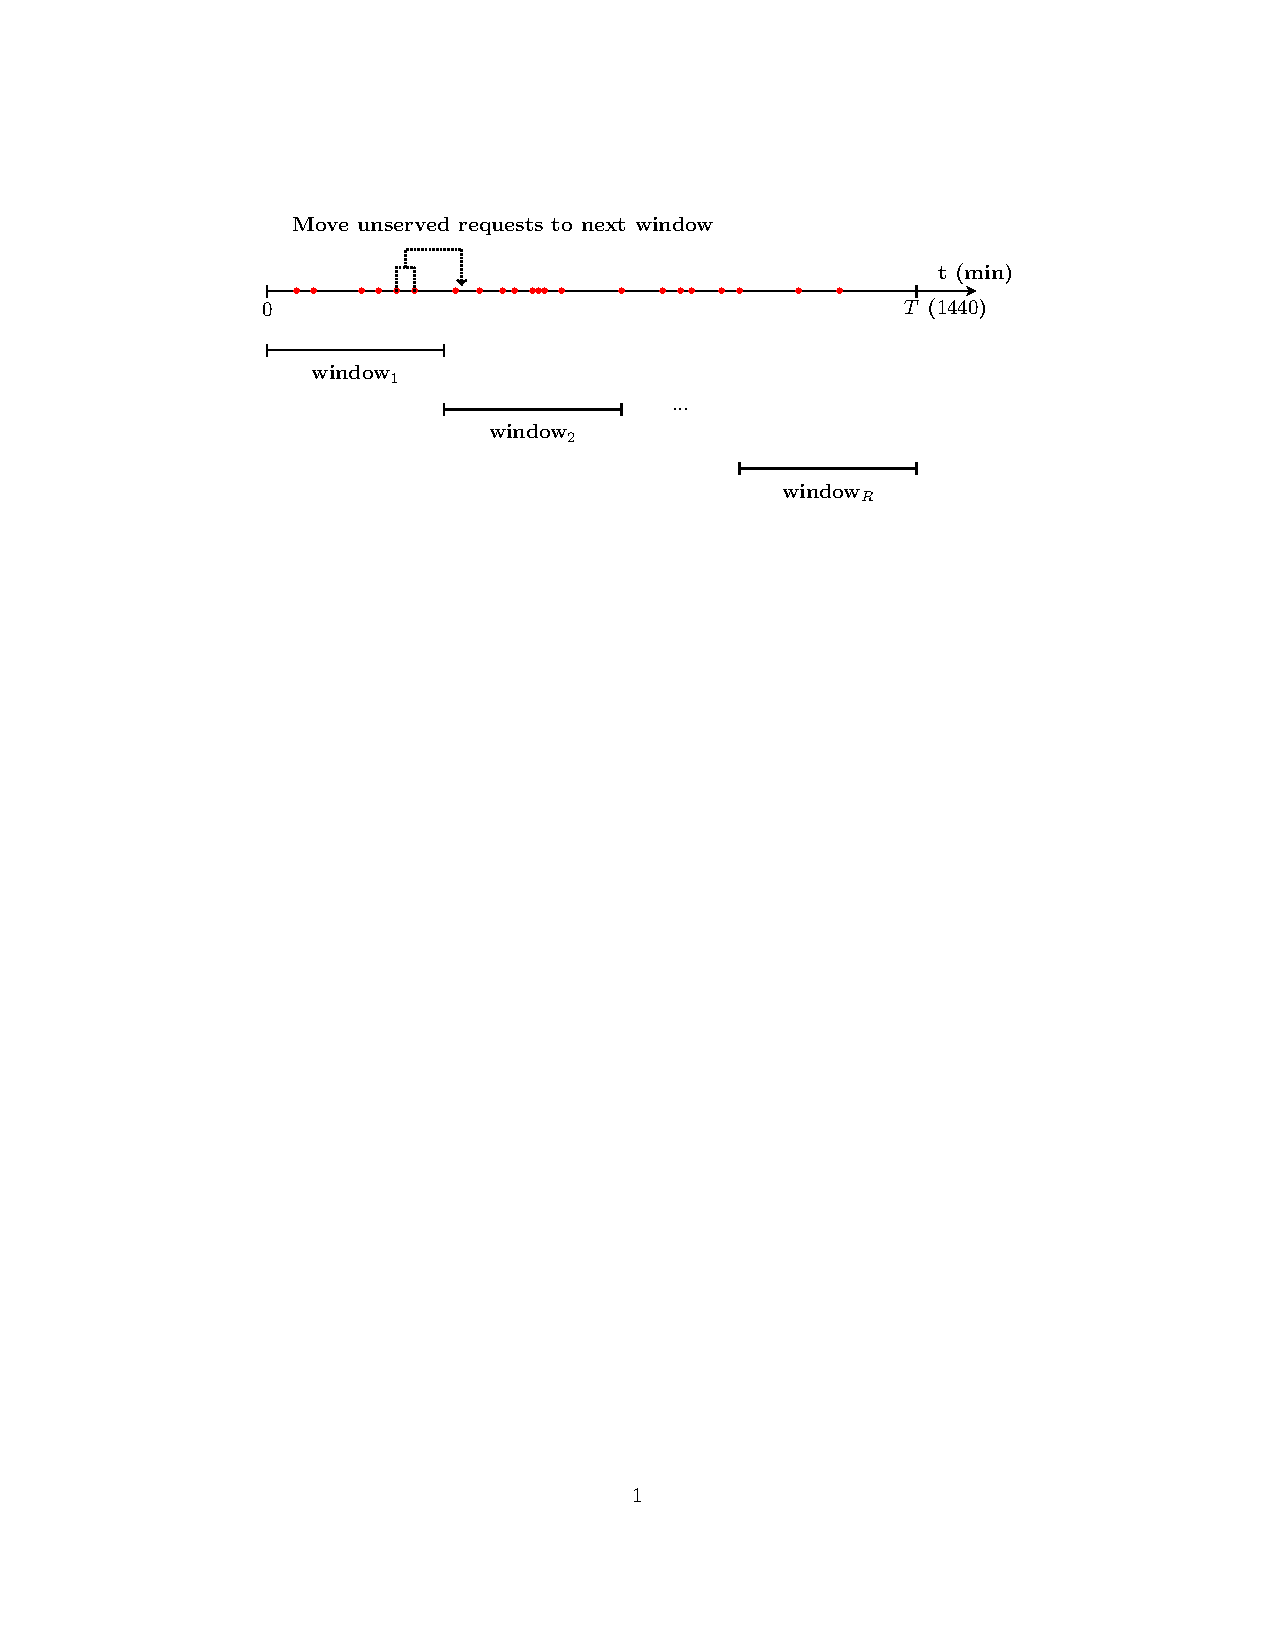
\includegraphics[trim=120 550 120 100,clip,width=0.85\textwidth]{images/rh-illustration.pdf}
	\caption{Rolling-horizon strategy with rolling time-windows.}
	\label{fig:rh}
\end{figure}

In the context of our \acs{RH} strategy, the (static) problem is solved in the first \textit{rolling window}, using a static scheduling heuristic (\acs{FCFS}, \acs{NN}, of the genetic algorithm of~\cite{panwadee2021}). At the end of this window, the \acs{RH} strategy moves the unserved requests to the beginning of the next window, and schedules them together with the new available requests in this window, as explained in Algorithm~\ref{alg:rh}.

\begin{algorithm}
	\caption{Rolling-horizon algorithm}\label{alg:rh}
	\begin{algorithmic}
		\Statex 1. \textbf{initialize} problem parameters (available taxis, battery level, scheduling horizon, rolling-window length)
		
		\Statex 2. \textbf{initialize} served and unserved requests ($=\emptyset$)
		
		\Statex 3. \textbf{for} each \texttt{rolling window} \textbf{do}
		
		\hspace{1cm} 4. \textbf{compute} available requests
		
		\hspace{1cm} 5. \textbf{append} non-served requests to available requests
		
		\hspace{1cm} 6. \textbf{apply a static scheduling heuristic} to schedule 
		
		\hspace{1cm} the available requests
		
		\hspace{1cm} 7. \textbf{update} served and non-served requests
		
		\hspace{1cm} 8. \textbf{update} battery level
		
	\end{algorithmic}
\end{algorithm}

The three scheduling heuristics that we use to solve the static problem inside each time window are explained in the next three sections.


\subsection{First-Come, First-Served}
\label{subsec:fcfs}

The \acs{FCFS} heuristic serves the requests according to the order given by their pick-up times. Indeed, the demands are sorted according to the non-decreasing order of their pick-up times. The advanced requests are served (without considering their locations) on their pick-up times or in an interval -- defined by the user -- centered around the pick-up time. The process continues until no request is available.

To illustrate how this heuristic works, let us consider an example. Suppose we have an instance with $2$ available flying taxis and $6$ requests, indexed by $1$, $2$, ..., $6$. The pick-up times (\texttt{pick\_t}) of each request is displayed in Table~\ref{tab:fcfs-exp}. The rows named \og\texttt{dur\_t}\fg, \og\texttt{ori\_x}\fg, \og\texttt{ori\_y}\fg, \og\texttt{des\_x}\fg, and \og\texttt{des\_y}\fg represent the duration, the x and y coordinates of the origin location of the request, and the x and y coordinates of the destination location, respectively.
\begin{table}
	\centering
	\begin{tabular}{ccccccc}
		\toprule
		\texttt{index}  &1     &  2    &    3  &    4  &    5   &   6\\
		\midrule
		\texttt{pick\_t}&   803 & 53    &  1373 &  1319 &  1425 &   710\\
		\texttt{dur\_t} &  26.1 & 19.17 &  30.01& 18.89 & 19.77 & 23.89\\
		\texttt{ori\_x} & 17182 &  5807 & 10958 & 12710 &  9890 & 10726\\
		\texttt{ori\_y} &  5391 &   828 & 21818 &  2405 & 21282 & 13201\\
		\texttt{des\_x} &  5753 & 10202 & 21534 & 20022 & 11893 & 21323\\
		\texttt{des\_y} & 12415 &  7076 &  8931 &  3602 & 13390 & 17863\\	
		\bottomrule
	\end{tabular}
	\caption{Example of an instance with $6$ requests.}
	\label{tab:fcfs-exp}
\end{table}

The \acs{FCFS} scheduler sorts the above-mentioned requests in the non-decreasing order of the pick-up times, then serves them in the resulting order. The battery level is checked before each customer pick-up, and updated after each customer drop-off. The solution provided by the \acs{FCFS} scheduler for our example is showed in Figure~\ref{fig:example-fcfs}. The green and orange bars illustrate the taxi service to serve the request and the battery recharging, respectively. 
\begin{figure}[h!]
	\centering
	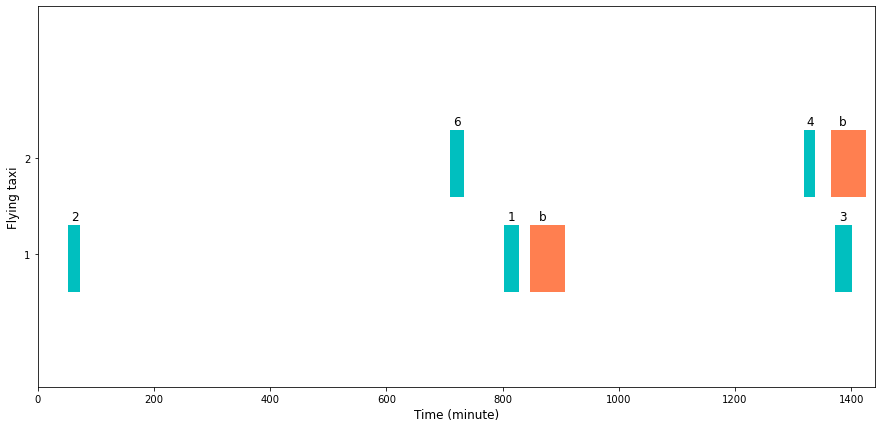
\includegraphics[width=0.9\textwidth]{images/example-fcfs}
	\caption{The \acs{FCFS} heuristic solution.}
	\label{fig:example-fcfs}
\end{figure}


\subsection{Nearest Neighbor}
\label{subsec:nn}

The \acs{NN} heuristic serves the closest requests to the current location of the taxi. Indeed, for each taxi, the \acs{NN} scheduler serves first the closest demand to the center. After completing service at the location of the first demand, the taxi travels to the nearest neighboring demand and so forth. The key difference between a \acs{FCFS} and a \acs{NN} scheduler is that the former sorts the customers at the beginning of the scheduling and then serves them, while the latter needs to compute the distances from current request location to all other unserved requests, to serve the closest one. This process is repeated after each customer drop-off to find the next one to serve. Hence, this heuristic may lead to larger computation times than the \acs{FCFS}.

If we consider the same example as in Section~\ref{subsec:fcfs}, the \acs{NN} heuristic solution is given in Figure~\ref{fig:example-nn}.

\begin{figure}[h!]
	\centering
	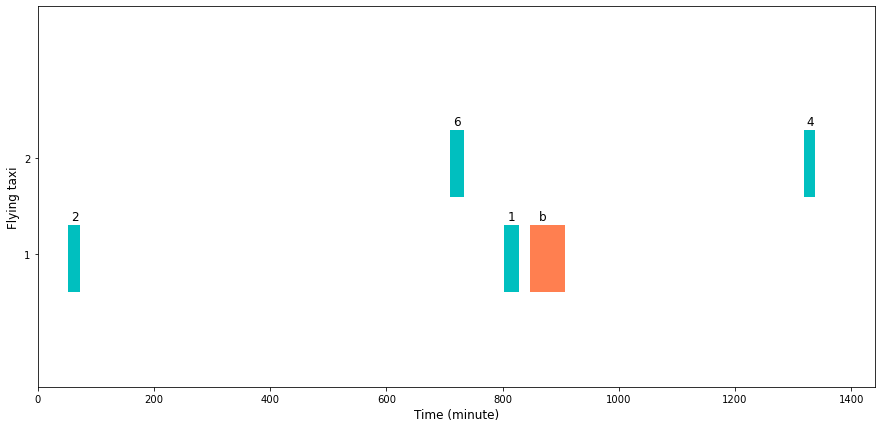
\includegraphics[width=0.9\textwidth]{images/example-nn}
	\caption{The \acs{NN} heuristic solution.}
	\label{fig:example-nn}
\end{figure}


\subsection{Genetic Algorithm}
\label{subsec:dynamic-ga}

The third heuristic that we integrate in the \acs{RH} approach is the \acs{GA} of~\cite{panwadee2021}, that was proposed to schedule flying taxis for the static case. In this \acs{GA}, the first population of chromosomes is randomly generated. Genetic operations such as mutations and crossovers are performed on this population, and best off-springs are selected to continue the process until the stopping criteria is satisfied. The latter corresponds to a number of iterations since the last improvement.

A chromosome is composed of genes whose values are randomly generated in the interval $[0,1]$.  Each gene represents a demand which is served by a flying taxi. Thus, the total number of genes in a chromosome is equal to the number of requests multiplied by the total number of taxis. For example, if we consider an instance with $3$ requests and $2$ flying taxis, the total number of genes is equal to $6$ (see Figure~\ref{fig:chromo})

\begin{figure}
	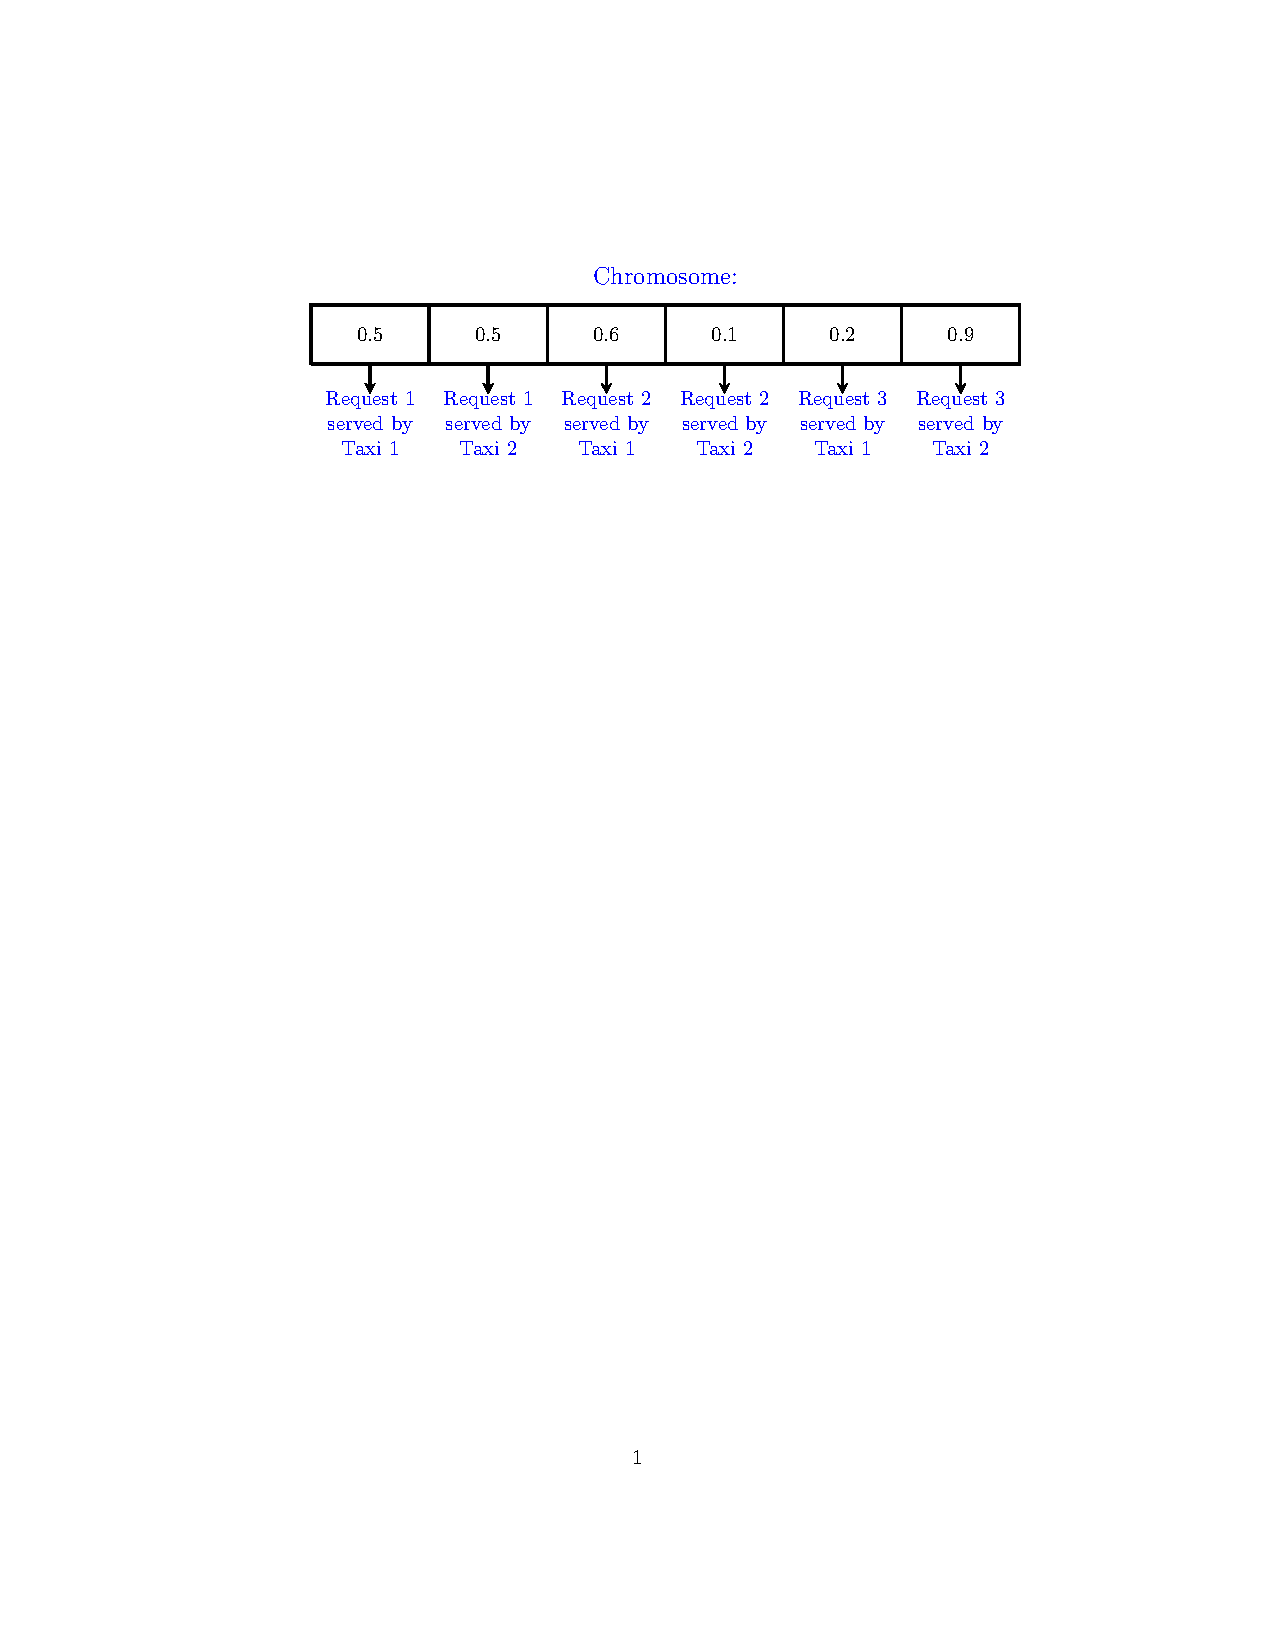
\includegraphics[trim=120 570 120 125,clip,width=0.85\textwidth]{images/chromosome.pdf}
	\caption{Example of a chromosome with six genes (3 requests/2 taxis).}
	\label{fig:chromo}
\end{figure}







	
	% Section 4

\section{Computational results and discussion}
\label{sec:results}

This section reports the computational results of implementing the above-mentioned heuristics, integrated in the \acs{RH} approach. All experiments are run on a computer under Windows operating system, processor Intel(R) Core(TM) i5-10310U with 8 GB of RAM. 

In section~\ref{subsec:instances}, we introduce new data-sets of instances that were generated based on~\cite{panwadee2021}. Our new instances are however more congested and feature more realistic aspect of the problem. Then, in Section~\ref{subsec:results-discussion} we present computational results of implementing our two heuristics \acs{FCFS} and \acs{NN}, and the \acs{GA} of~\cite{panwadee2021}, all integrated in a \acs{RH} approach.


\subsection{New generated instances}
\label{subsec:instances}

We randomly generate $10$ test instances, based on the instance generator of~\cite{panwadee2021}. In addiction to being more congested, our instances define a time window for each request during which it can be served, which is more realistic that imposing a strict pick-up time.

Table~\ref{tab:instances} summarizes some important characteristics of our generated instances. Throughout this table, the first, second and third columns present the name, the total number of requests, and the total number of air taxis in each instance (respectively). The fourth column \og req/h\fg  reports the average request per hour in each instance, which measures how dense the latter is. The remaining columns show the minimum, average, and the maximum duration of request trips in an instance. 

\begin{table}[ht]
	\resizebox{0.99\linewidth}{!}{%
		\begin{tabular}{p{3cm}rrrp{2cm}p{1.2cm}p{1.2cm}}
			\toprule
			Instance name &  \#\newline req & \#\newline taxis & req/h &
			min\newline duration & average\newline duration &
			max\newline duration \\
			\midrule
			\texttt{instance50\_2}    &50   &2 &2.08  &12.75& 27.12& 49.07\\
			\texttt{instance100\_3}   &100  &3 &4.17  &11.00& 26.8 & 48.57\\
			\texttt{instance100\_5}   &100  &5 &4.17  &11.71& 26.75& 51.37\\
			\texttt{instance250\_5}   &250  &5 &10.42 &10.42& 27.7 & 47.48\\
			\texttt{instance250\_10}  &250  &10&10.42 &10.42& 27.70& 49.48\\
			\texttt{instance500\_4}   &500  &4 &20.83 &10.51& 26.57& 47.85\\
			\texttt{instance500\_10}  &500  &10&20.83 &10.48& 27.26& 49.15\\
			\texttt{instance1000\_9}  &1000 &9 &41.67 &10.33& 26.96& 49.74\\
			\texttt{instance1000\_15} &1000 &15&41.67 &10.49& 27.16& 49.35\\
			\texttt{instance10000\_20}&10000&20&416.66&10.16& 27.01& 52.85\\
			\bottomrule
		\end{tabular} 
	}
	\caption{Characteristics of the new constructed instances.}
	\label{tab:instances}
\end{table}

The data included in our instances contain the request identifier, the origin and destination locations of the requests and their pick-up times. Moreover, we define for each request a time window in which it can be served. The time window is defined by an earliest and a latest serving time, centered around the pick-up time.  


\subsection{Results and discussion}
\label{subsec:results-discussion}

To compare the quality of the solutions provided by the above-mentioned heuristics, we define the following performance indicators:
\begin{itemize}
	\item The \textbf{objective-value} that indicates the total service time (in minutes). In an optimization approach, this objective is maximized.
	
	\item The \textbf{non-profitable trips} duration that corresponds to the total travel time without passengers. This may occur when a taxi flies to the center to recharge its battery, or between two requests. In an optimization approach, this indicator should be minimized. 

	\item The \textbf{CPU} time that indicates the computation times in seconds. The characteristics of the computer on which the experiments were run are provided at the beginning of Section~\ref{sec:results}.
\end{itemize}

Figure(reference here) shows...














	
	

\section{Conclusion and future tracks of research}

	
	%%%%%%%%%%%%%%%%%%%%%%%%%%%
	%%% Referenvces are included here 
	%%%%%%%%%%%%%%%%%%%%%%%%%%%
	\clearpage
	\printbibliography
	
	
	
	
	%%%%%%%%%%%%%%%%%%%%%%%%%%%
	%%% Appendices are included here 
	%%%%%%%%%%%%%%%%%%%%%%%%%%%
	\clearpage
	\appendix
	%\let\clearpage\relax
	%\mbox{~}
	% First Appendix

\section{Abbreviations and Acronyms}


\begin{acronym}[CP-OFDMX]

\acro{EdC}{Élément de Compréhension}

\acro{FCFS}{First-Come, First-Served}

\acro{GA}{Genetic Algorithm}
	
\acro{JSSP}{Job-Shop Scheduling Problem}

\acro{NN}{Nearest Neighbor}

\acro{RH}{Rolling Horizon}
	
\acro{UAM}{Urban Air Mobility}

\acro{UAV}{Unmanned Aerial Vehicle}

\acro{VRP}{Vehicle Routing Problem}

\end{acronym}

	
	
	
	
	
\end{document}


